% !TeX root = Bericht.tex
% !TeX spellcheck = en_US
\section{Results}
We start by analyzing the lasers beam parameters by recording the beams radius $w$ at different distances $z$. The latter was measured using a millimeter-scale ruler with chosen uncertainty of $1 \unit{mm}$. Due to some fluctuations in the waistmeter's reading, we chose the uncertainty to be $3 \unit{\micro\m}$, which could be reduced by taking multiple readings and averaging. 11 datapoints were taken in steps of $1.5 \unit{cm}$ and can be seen in \autoref{fig:w1}. Additionally, a function following \autoref{eqn:wz} was fitted and can be seen as solid orange line, accompanied by a $1\sigma$ confidence band. 

\begin{figure}[H]
	\centering
	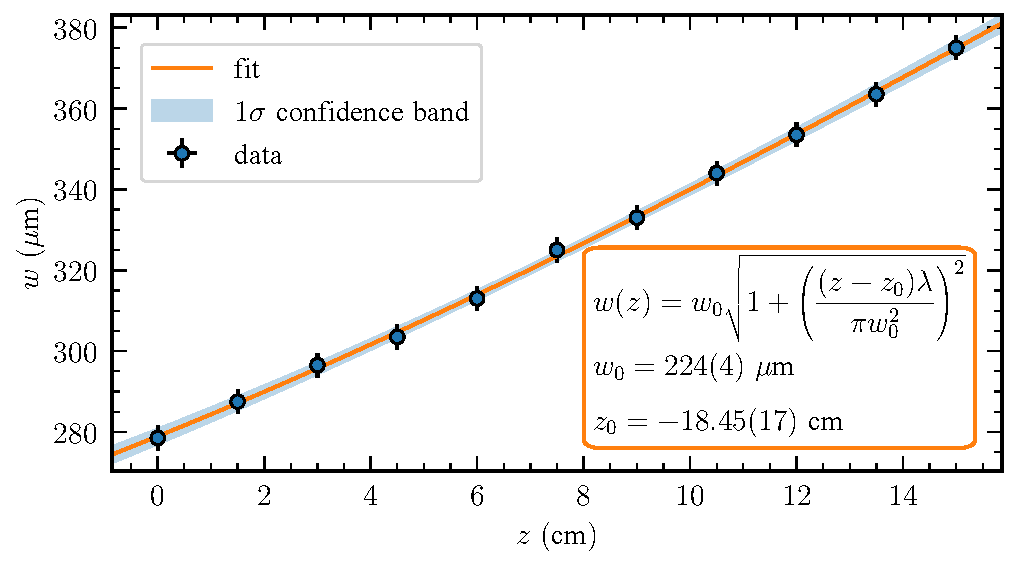
\includegraphics[width=\textwidth]{w1}
	\caption{The measured beam radius $w$ of freely propagating laser light is plotted against the distance $z$. A function was fitted and can be seen as orange line and is surrounded by a $1\sigma$ confidence band. The fitfunction and according parameters can be seen in the bottom right. Errorbars denote $1\sigma$ uncertainties with the errors in x-direction being too small to make out.}
	\label{fig:w1}
\end{figure}

In \autoref{fig:w1}, we can see that the data nicely follows theory (all datapoints are within $1\sigma$ of the fitted curve). We can extract a beam waist $w_0 = 224(4) \unit{\micro\m}$ at a focus position of $z_0 = -18.45(17) \unit{mm}$, which approximately lies at the end of the laser housing.

Before using the determined beam waist to match it to a cavity, we analyzed the effect of a lens with focal length $f = 100 \unit{mm}$ on the beam radius. Again, data was taken in intervals of $1.5 \unit{cm}$ with the same uncertainties as described above. The data with an appropriate fit can be seen in \autoref{fig:w2}. Here a $2\sigma$ confidence band was chosen, to help gauge the deviation of the datapoints from the fit line around the focus point.

\begin{figure}[H]
	\centering
	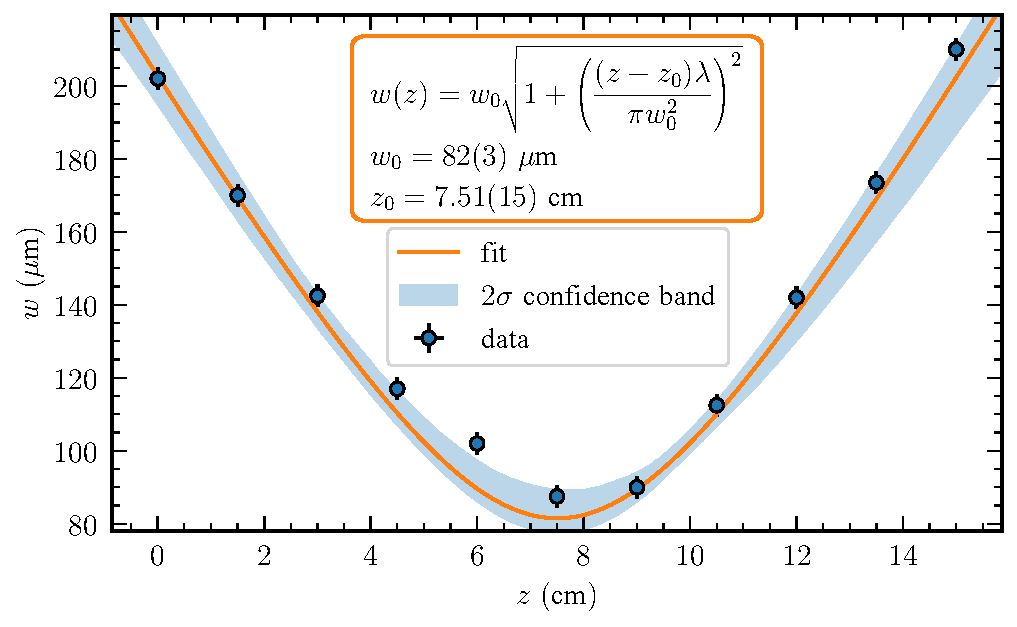
\includegraphics[width=\textwidth]{w2}
	\caption{The measured beam radius $w$ of laser light after a lens with $f = 100 \unit{mm}$ is plotted against the distance $z$. A function was fitted and can be seen as orange line and is surrounded by a $2\sigma$ confidence band. The fitfunction and according parameters can be seen in the bottom right. Errorbars denote $1\sigma$ uncertainties with the errors in x-direction being too small to make out.}
	\label{fig:w2}
\end{figure}

The data in \autoref{fig:w2} mostly follows the expected behavior, with outliers around the focus point $z_1 = 7.51(15) \unit{cm}$. This could have been caused by the waistmeter being slightly tilted against the laser's propagation axis, leading to higher radius measurements. After adding the distance between the closest radius measurement and the lens, which was estimated to be $2.5(2) \unit{cm}$, $f_{\mathrm{exp}} = 100(2) \unit{mm}$ is in good agreeance with $f_{\mathrm{lens}} = 100 \unit{mm}$. As for the waist, using the matrix formalism described in \autoref{subsec:matrix} we can get a theoretical prediction for the beam waist after a lens. Comparing the exact theoretical result with the experimental value
$$ w_{1, \mathrm{theo}} = 83.3(1.1) \unit{\micro\m} \qquad w_{1,\mathrm{exp}} = 82(3) \unit{\micro\m}, $$ 
we conclude that our experiment is consistent with theory. The approximating $w_1 = f\lambda/\pi w_0$ yields a value of $89.7(1.6) \unit{\micro\m}$, which deviates significantly from both, experimental and exact theoretical result. It is therefore not appropriate to use this approximation on a lens with focal length $f = 100 \unit{mm}$. 

After matching the lasers beam waist to that of the cavity (for a detailed procedure see \autoref{subsec:mode}), we can validate the confocal condition (mirror curvature $r$ equal mirror distance $L$) by measuring the distance to half axial modes. For this the transmitted laser signal was recorded on the oscilloscope and normalized using the highest datapoint (normalization was done for convenience). Then we isolate the peaks intended for studying and we fit a multilorentzian function (sum of multiple Lorentz functions with independent parameters) to the data. By calculating the free spectral range of the cavity $\nu_{\mathrm{FSR}} = c/2L = 1 \unit{GHz}$ and the fitted distance between peaks of the same height, we can convert the time domain measurement from the oscilloscope to frequencies. The fit also lets us compute the distance between \blockquote{regular} and half axial modes. All this can be seen in \autoref{fig:multilorentzian}.

\begin{figure}[H]
	\centering
	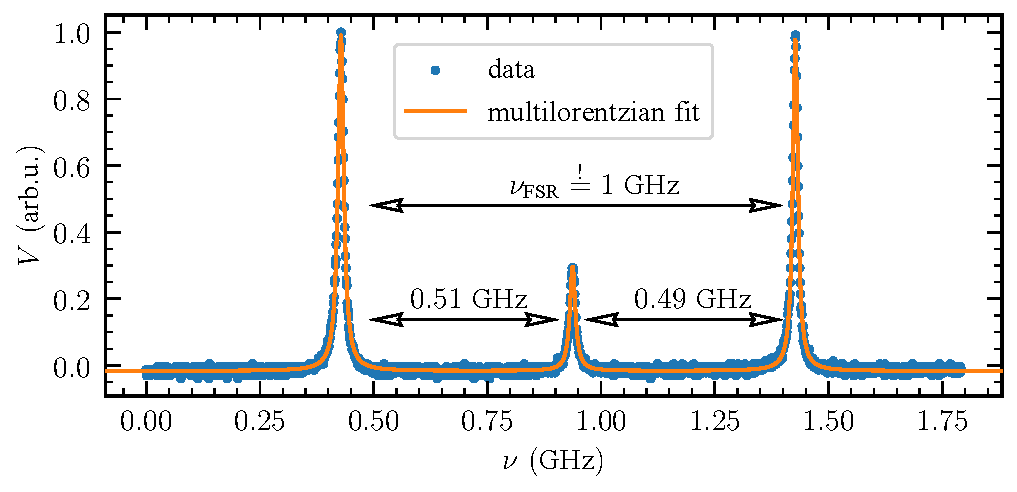
\includegraphics[width=\textwidth]{multilorentzian}
	\caption{The recorded signal amplitude $V$ is plotted against the frequency $\nu$. A fit function consisting of three independent Lorentz functions was fitted and can be seen as solid line. The distance between the two $\mathrm{TEM}_{00}$ peaks was used to calibrate the x-Axis, while the distance to the half axial peak, seen in the middle was determined from fit parameters.}
	\label{fig:multilorentzian}
\end{figure}

As can be seen in \autoref{fig:multilorentzian}, the confocal condition is almost met, with distances of $0.49 \unit{GHz}$ and $0.51 \unit{GHz}$. Statistical errors are omitted, since the fit returned values in the range of $\oldunit{kHz}$, at which systematical errors probably play a critical role. 

Having confirmed the cavity to be confocal, we can optimize the mirrors to maximize the mode's intensity (by reducing the half axial mode's intensity). We then repeat the same procedure seen in \autoref{fig:multilorentzian}, with the only difference being that we recorded and fitted four Lorentz functions. We can evaluate the finesse $\mathcal{F}$ for each Lorentz peak using \autoref{eqn:finesse} and the fitted full width at half minimum (FWHM). Assuming a mirror reflectivity of $R = 98\%$ and mirror transmission being the only losses, we can compute a theoretical upper limit for the finesse. Below are the theoretical limit and a mean of experimentally determined finesse values:
$$ \mathcal{F}_{\text{theo}} = 155.50  \qquad \mathcal{F}_{\text{exp}} = 75.91(15) $$
It is apparent, that other loss mechanisms are at play in the system.

So far, we have only studied TEM$_{00}$ and TEM$_{01}$ modes. We can go to higher modes by increasing the cavity's length by $13.53(1) \unit{mm}$ and exiting the confocal condition. We study higher modes qualitatively, by taking pictures with a CCD camera. The pictures are plotted in \autoref{fig:gaussmodes}. Additionally, we converted the images to grayscale and used it as proxy for the beam's intensity. This allows us, to project the image onto the horizontal and vertical axis by summing over the images rows and columns. We can fit Hermite-Gaussian functions of the appropriate order to the projections. Both data (black) and fit (red) are plotted on the marginal axes in \autoref{fig:gaussmodes}.

\begin{figure}[H]
	\centering
	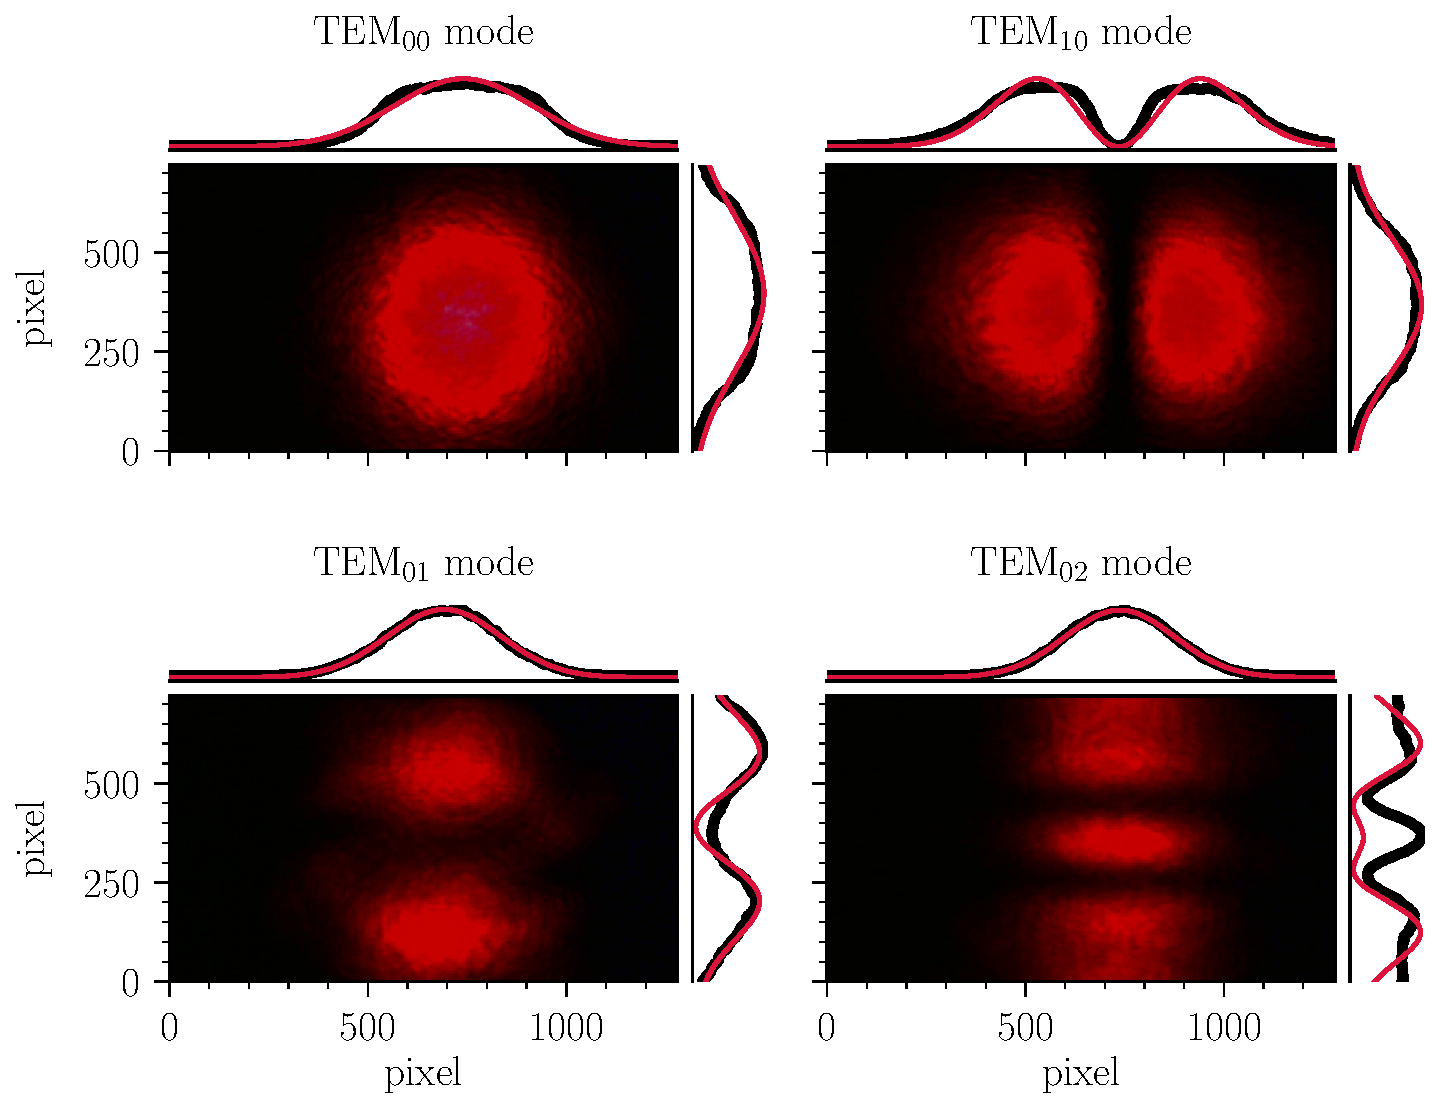
\includegraphics[width=\textwidth]{gaussmodes}
	\caption{Four images of different TEM modes are depicted on a per-pixel basis. All of them are accompanied by marginal axes, onto which the intensity is projected and shown as black datapoints. The red lines represent fitted Hermite-Gaussian polynomials.}
	\label{fig:gaussmodes}
\end{figure}

Looking at \autoref{fig:gaussmodes}, we can clearly identify TEM$_{00}$, TEM$_{10}$ and TEM$_{01}$ modes, with projected intensities matching the fitted Hermite-Gaussian function. The TEM$_{02}$ mode (or possibly higher) is vertically not completely captured by the CCD camera, which makes fitting to difficult. In the top two pictures we saturate the CCD's recordable brightness. This can be directly observed in the optical picture as color discontinuity towards the center of the laser beam, further supported by a plateauing off toward the maximal intensity in all marginal projections. 

Lastly, we recorded a spectrum of higher order modes to compare the distance between modes with \autoref{eqn:cos}. Again, the data with calibrated x-Axis and fitted lorentzians can be seen in \autoref{fig:multilorentzian2}. 

\begin{figure}[H]
	\centering
	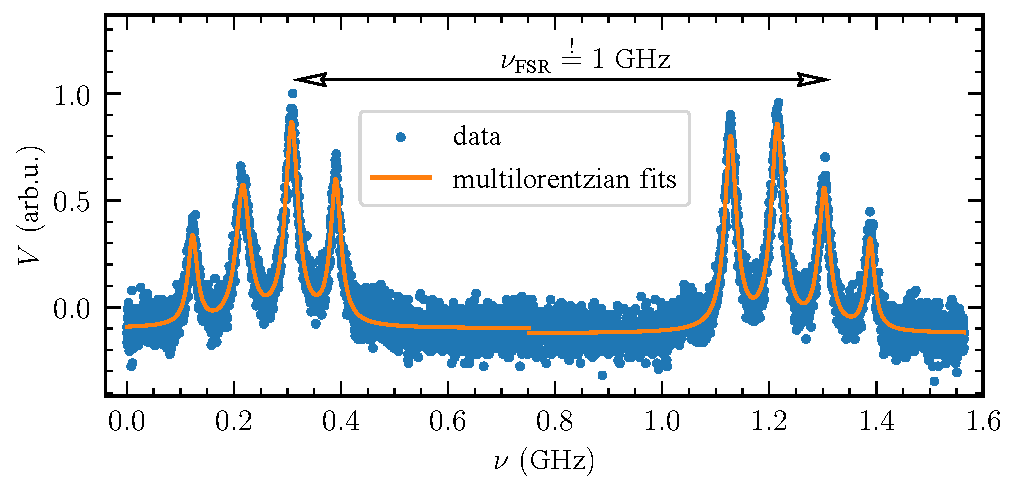
\includegraphics[width=\textwidth]{multilorentzian2}
	\caption{The recorded signal amplitude $V$ is plotted against the frequency $\nu$. The data was split in equal halves, to which functions consisting of four independent Lorentz functions were fitted and can be seen as solid orange lines. The distance between the third peaks from the left was used to calibrate the x-Axis, while the distance to the half axial peak, seen in the middle was determined from fit parameters.}
	\label{fig:multilorentzian2}
\end{figure}

From the fits, we get a mean mode spacing of $\Delta\nu = 88.03(8) \unit{MHz}$. From the theory side, replacing the mirror spacing $L = 150 \unit{mm}$ in confocal setup with the new length of $L = 163.53(1) \unit{mm}$, $\arccos(1 - L/r)/\pi$ increases from exactly $0.5$ to $0.529(2)$. This leads to a shift in frequency for higher modes ($m,n > 0$) with increasing $q$, as can be seen in \autoref{fig:spektrum_cavities}. However, the predicted fundamental mode spacing of $29(2) \unit{MHz}$ is too small to explain the data. Only moving to modes with $m+n = 2$ (this effectively rescales the output of the $\arccos$), the predicted mode spacing becomes $86(6) \unit{MHz}$. Whilst in good agreeance with experimental results, it requires dominant TEM$_{mn}$ modes with $m+n = 2$. Although possible, it is quite unlikely that we do not simultaneously excite higher or lower modes. It is also possible, that we did not observe a full FSR of the cavity with the recorded data still representing substructures, rendering our x-Axis calibration false. 










